\begin{frame}{Поиск доказательств}

    Система доказательств $\Pi$ автоматизируема $\Rightarrow$ существует алгоритм $A$:
    \begin{itemize}
        \item $\varphi \in \UNSAT, A(\varphi) = w \Rightarrow \Pi(\varphi, w) = 1$;
        \item $A$ полиномиален от $|\varphi|$ и $\min\limits_{|w'|} \{w' \mid \Pi(\varphi, w') = 1\}$.
    \end{itemize}

    \pause
    Некоторые результаты:
    \begin{itemize}
        \item{} [Алехнович, Разборов 08] $\FPT \neq \langcplx{W}[1] \Rightarrow$ резолюция
            неавтоматизируема.
            \pause
        \item{} [Atserias, M{\"{u}}ller 19] $\P \neq \NP \Rightarrow$ резолюция неавтоматизируема.
            \pause
        \item{} [de Rezende et al. 21] $\P \neq \NP \Rightarrow$ Nullstellensatz и ряд других
            алгебраических систем неавтоматизируемы.
    \end{itemize}
\end{frame}

\begin{frame}{Некоторые открытые вопросы}

    \deftext{Polynomial Calculus} ($\PCR[\field]$) доказательство несовместности системы равенств $\Fs
    \coloneqq \{f_1 = 0, f_2 = 0, \dots, f_m = 0\}$~--- это последовательность полиномов $(p_1, p_2, p_3,
    \dots, p_{\ell})$:
    \pause
    \begin{enumerate}
        \item $p_i \in \Fs \cup \bigcup\limits_{j = 1}^{n} \{x_i^2 - x_i\}$;
        \pause
        \item $p_i = x_j p_k$ для некоторого $j$ и $k < i$;
        \pause    
        \item $p_i = \alpha p_k + \beta p_s$ для некоторых $k, s < i$ и $\alpha, \beta \in \field$;
        \pause
        \item $p_{\ell} = 1$.
    \end{enumerate}
    



    \begin{itemize}
        \item Какова сложность $\PHP_n^{n^3}$ в системе $\PCR[\field]$.
            \pause
        \item Нижние оценки на систему $\PrSys{Frege}$.
        \item Какова сложность случайных $\Delta$-КНФ формул в системах $\CP$ и
            $\AC[0]\text{-}\PrSys{Frege}$.
    \end{itemize}

\end{frame}


\begin{frame}{Коммуникационные протоколы. $f\colon U \times V \to T$}
    \begin{center}
    	\onslide<1->{
    \tikzstyle{op1} = [opacity = 0]
    \tikzstyle{op2} = [opacity = 0]
    \tikzstyle{op3} = [opacity = 0]
    \tikzstyle{op4} = [opacity = 0]
}
\only<2->{\tikzstyle{op2} = [opacity = 1]}
\only<3->{\tikzstyle{op3} = [opacity = 1]}
\only<4->{\tikzstyle{op4} = [opacity = 1]}

\begin{tikzpicture}[black]
    \node[police, female, minimum size = 1.5cm] (alice) at (0, 0) {};
    \node[jester, mirrored, minimum size = 1.5cm] (bob) at (7, 0) {};
    \node[above = 0.3 of alice] {$x \in U$};
    \node[above = 0.3 of bob] {$y \in V$};

    \path (alice.east) -- (bob.west) node[midway, above = 2.3] {\Large $f(x, y) = ?$};
    \draw[op2, ->, thick] ($(alice.east) + (0.3, 1)$) -- ($(bob.west) + (-0.3, 1)$) node[midway, above] {$r_1 = a(x)$};
    \draw[op3, <-, thick] ($(alice.east) + (0.3, 0.2)$) -- ($(bob.west) + (-0.3, 0.2)$) node[midway, above] {$r_2 = b(y,
        r_1)$};
    \draw[op4, ->, thick] ($(alice.east) + (0.3, -0.2)$) -- ($(bob.west) + (-0.3, -0.2)$);
    \draw[op4, ->, thick] ($(alice.east) + (0.3, -0.6)$) -- ($(bob.west) + (-0.3, -0.6)$) node[midway, below] {$\vdots$};
\end{tikzpicture}    
    \end{center}

    \pause
    \pause
    \pause
	\pause

    \begin{itemize}
        \item Глубина~--- число раундов (в худшем случае).
        \item $\DCC(f) = \min\limits_{P \in \mathcal{P}} \mathrm{depth}(P)$, где $\mathcal{P}$~---
            множество протоколов для $f$.
    \end{itemize}
\end{frame}

\begin{frame}{Протоколы и деревья}

    Алиса полуает $u \in U$, Боб $v \in V$. Протокол~--- это дерево:

    \begin{columns}[t]
		\begin{column}{0.7\textwidth}
            \begin{itemize}
                \item<2-> вершины помечены игроками;
    		    \item<7-> листья ответами.
	        \end{itemize}

    	%	\onslide<8->{
        %        Size of protocol is a size of the tree. $\mathrm{Size}(f) = \min\limits_{P \in
        %            \mathcal{P}} \mathrm{Size}(P)$.
        %    }
        %    \onslide<9->{
        %        \begin{lemma}
        %            $\DCC(f) = \Omega(\log(\mathrm{Size}(f)))$.
        %        \end{lemma}
        %    }
        \end{column}
        
		\begin{column}{0.25\textwidth}
            \tikzstyle{inner} = [thin, circle, minimum size = 0.3cm, draw, inner sep = 0.1pt, black]
\tikzstyle{inner_g} = [thin, circle, minimum size = 0.3cm, draw, inner sep = 0.1pt, black, fill = green]
\tikzstyle{inner_r} = [thin, circle, minimum size = 0.3cm, draw, inner sep = 0.1pt, black, fill = red]
\tikzstyle{inner_b} = [thin, circle, minimum size = 0.3cm, draw, inner sep = 0.1pt, black, fill = blue!50!white]
\tikzstyle{ed} = [thick, ->, draw, black]

    
\begin{tikzpicture}
    \only<-3, 5->{
        \node[inner] (a) at (0, 0) {\scriptsize $a$};
	}
    \only<4>{
        \node[inner_g] (a) at (0, 0) {\scriptsize $a$};
    }

    \only<-4, 6->{
        \node[inner] (b) at (-0.9, -1.2) {\scriptsize $b$};
	}
    \only<5>{
        \node[inner_g] (b) at (-0.9, -1.2) {\scriptsize $b$};
    }

    \node[inner] (c) at (0.9, -1.2) {\scriptsize $a$};
    \node[inner, label = below:$t_1$] (d) at (-1.5, -2.4) {};

    \only<-5, 7->{
        \node[inner] (e) at (-0.3, -2.4) {\scriptsize $b$};
	}
    \only<6>{
        \node[inner_g] (e) at (-0.3, -2.4) {\scriptsize $b$};
    }

    \node[inner] (e2) at (0.3, -2.4) {\scriptsize $b$};
    \node[inner, label = below:$t_4$] (f) at (1.5, -2.4) {};

    \only<-6, 9->{
        \node[inner, label = below:$t_2$] (g) at (-1.5, -4.3) {};
	}
    \only<7-8>{
        \node[inner_g, label = below:$t_2$] (g) at (-1.5, -4.3) {};
    }
    
    \node[inner, label = below:$t_3$] (h) at (-0.25, -4.3) {};
	\node[inner, label = below:$t_3$] (g2) at (1.5, -4.3) {};
    \node[inner, label = below:$t_2$] (h2) at (0.25, -4.3) {};
    
    \path (a) edge[ed] (b);
    \path (a) edge[ed] (c);
    \path (b) edge[ed] (d);
    \path (b) edge[ed] (e);
    \path (c) edge[ed] (e2);
    \path (c) edge[ed] (f);
    \path (e) edge[ed] (g);
    \path (e) edge[ed] (h);
    \path (e2) edge[ed] (g2);
    \path (e2) edge[ed] (h2);
\end{tikzpicture}

		\end{column}
	\end{columns}

\end{frame}

\begin{frame}{Отношение $\KW$ [Karchmer, Wigderson 90]}
    $U, V \subseteq \{0, 1\}^{n}$ и $U \cap V = \emptyset$.

    \vspace{0.1cm}
    $\KW$:
    \begin{itemize}
        \item Алиса получает $u \in U$, Боб получает $v \in V$;
        \item цель: найти такой $i$, что $u_i \neq v_i$.
    \end{itemize}
    \pause
    Монотонная версия $\KWm$:
    \begin{itemize}
        \item цель: найти такой $i$, что $u_i = 1 \land v_i = 0$.
    \end{itemize}

    \pause

    \begin{theorem}[Karchmer, Wigderson 90]
        \alert{Монотонная} формула для $f$ размера $S$ $\Leftrightarrow$ коммуникационный протокол для
        \alert{$\KWm$} $\KW$ размера $S$, где $U \coloneqq f^{-1}(1), V \coloneqq f^{-1}(0)$. 
    \end{theorem}
\end{frame}


\begin{frame}{$\Search_{\varphi}$ [Lov{\'{a}}sz, Naor, Newman, Wigderson et al. 94]}
    
    $\varphi(z) \coloneqq \bigvee\limits_{i = 1}^{m} C_i$ невыполнимая КНФ формула.
    \pause
    
    $\Search_{\varphi} \subseteq \{0, 1\}^n \times [m]$:
    \begin{itemize}
        \item $(\alpha, i) \in \Search_{\varphi} \Leftrightarrow C_{i}(\alpha) = 0.$
    \end{itemize}

    \pause
    \vspace{0.1cm}
    Коммуникационная версия:
    \begin{itemize}
        \item ``gadget'' $g\colon X \times Y \to \{0, 1\}$;
        \item $\Ind\colon [k] \times \{0, 1\}^k \to \{0, 1\}$, $\Ind(x, y) = y_x$.
    \end{itemize}

    \pause
    \begin{center}
        \begin{tikzpicture}
    \node[thick, circle, draw] (S) at (0, 0) {\Large $S$};
    
    \foreach \i in {1, 2, ..., 5}{
        \node (z\i) at (-3 + \i, -1.5) {$z_{\i}$};
        \draw[->] (z\i) -- (S);
    }
    
    \node[minimum height = 1cm, single arrow, draw] at (3, 0) {composition};

    \node[thick, circle, draw] (S1) at (6, 0) {\Large $S$};

    \foreach \i in {1, 2, ..., 5}{
        \node[draw, circle] (i\i) at (3 + \i, -1.5) {\scriptsize $g$};
        \draw[->] (i\i) -- (S1);

        \node (x\i) at (2.75 + \i, -2.4) {\scriptsize $x_{\i}$};
        \node (y\i) at (3.25 + \i, -2.4) {\scriptsize $y_{\i}$};
        \draw[->] (x\i) -- (i\i);
        \draw[->] (y\i) -- (i\i);
    }
\end{tikzpicture}
    \end{center}


    $\Search_{\varphi} \circ g \equiv \Search_{\varphi \circ g}$.
\end{frame}

\begin{frame}{Lifting 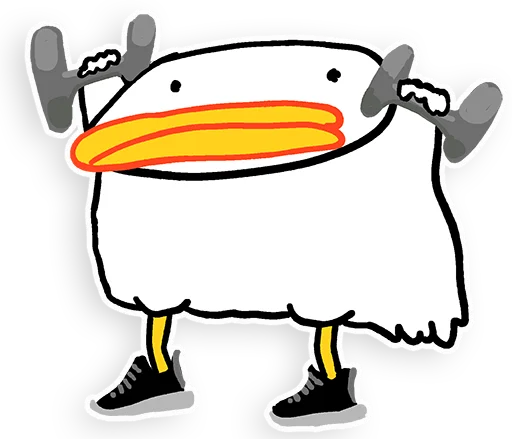
\includegraphics[scale = 0.04]{pics/utia-lift.png}}

    \begin{theorem}[Raz, McKenzie 99; G\"{o}\"{o}s, Pitassi, Watson 16]
        Резолюционная глубина $\varphi$ не менеее $d$ $\Rightarrow$
        $\DCC(\Search_{\varphi} \circ \Ind_m) \ge n^{\bigO{d}},$
        где $m \coloneqq \poly(n)$. \alert{$\DCC(\Search_{\varphi} \circ \Ind_m) \approx
            \DCC(\Ind) \cdot \mathrm{res\text{-}depth}(\varphi)$.}
    \end{theorem}

    Следствие: нижние оценки на монотонные формулы $2^{n^{\varepsilon}}$.
    \pause

    \begin{theorem}[Garg, G\"{o}\"{o}s, Kamath, S 18]
        Резолюционный размер $\varphi$ не менее  $S$ $\Rightarrow$
        размер \alert{dag-like} протокола для $\Search_{\varphi} \circ \Ind_m$ не менее $\Omega(S),$
        where $m \coloneqq \poly(n)$.
    \end{theorem}

        Следствие: нижние оценки на монотонные \textcolor{blue}{схемы} $2^{n^{\varepsilon}}$.
    \pause

    \begin{theorem}[Pitassi, Robere 16; Robere, Pitassi 18, informal]
        Nullstellensatz $\Leftrightarrow$ \alert{algebraic tiling} для $\Search_{\varphi} \circ g$.
    \end{theorem}

\end{frame}